\documentclass[1p]{elsarticle_modified}
%\bibliographystyle{elsarticle-num}

%\usepackage[colorlinks]{hyperref}
%\usepackage{abbrmath_seonhwa} %\Abb, \Ascr, \Acal ,\Abf, \Afrak
\usepackage{amsfonts}
\usepackage{amssymb}
\usepackage{amsmath}
\usepackage{amsthm}
\usepackage{scalefnt}
\usepackage{amsbsy}
\usepackage{kotex}
\usepackage{caption}
\usepackage{subfig}
\usepackage{color}
\usepackage{graphicx}
\usepackage{xcolor} %% white, black, red, green, blue, cyan, magenta, yellow
\usepackage{float}
\usepackage{setspace}
\usepackage{hyperref}

\usepackage{tikz}
\usetikzlibrary{arrows}

\usepackage{multirow}
\usepackage{array} % fixed length table
\usepackage{hhline}

%%%%%%%%%%%%%%%%%%%%%
\makeatletter
\renewcommand*\env@matrix[1][\arraystretch]{%
	\edef\arraystretch{#1}%
	\hskip -\arraycolsep
	\let\@ifnextchar\new@ifnextchar
	\array{*\c@MaxMatrixCols c}}
\makeatother %https://tex.stackexchange.com/questions/14071/how-can-i-increase-the-line-spacing-in-a-matrix
%%%%%%%%%%%%%%%

\usepackage[normalem]{ulem}

\newcommand{\msout}[1]{\ifmmode\text{\sout{\ensuremath{#1}}}\else\sout{#1}\fi}
%SOURCE: \msout is \stkout macro in https://tex.stackexchange.com/questions/20609/strikeout-in-math-mode

\newcommand{\cancel}[1]{
	\ifmmode
	{\color{red}\msout{#1}}
	\else
	{\color{red}\sout{#1}}
	\fi
}

\newcommand{\add}[1]{
	{\color{blue}\uwave{#1}}
}

\newcommand{\replace}[2]{
	\ifmmode
	{\color{red}\msout{#1}}{\color{blue}\uwave{#2}}
	\else
	{\color{red}\sout{#1}}{\color{blue}\uwave{#2}}
	\fi
}

\newcommand{\Sol}{\mathcal{S}} %segment
\newcommand{\D}{D} %diagram
\newcommand{\A}{\mathcal{A}} %arc


%%%%%%%%%%%%%%%%%%%%%%%%%%%%%5 test

\def\sl{\operatorname{\textup{SL}}(2,\Cbb)}
\def\psl{\operatorname{\textup{PSL}}(2,\Cbb)}
\def\quan{\mkern 1mu \triangleright \mkern 1mu}

\theoremstyle{definition}
\newtheorem{thm}{Theorem}[section]
\newtheorem{prop}[thm]{Proposition}
\newtheorem{lem}[thm]{Lemma}
\newtheorem{ques}[thm]{Question}
\newtheorem{cor}[thm]{Corollary}
\newtheorem{defn}[thm]{Definition}
\newtheorem{exam}[thm]{Example}
\newtheorem{rmk}[thm]{Remark}
\newtheorem{alg}[thm]{Algorithm}

\newcommand{\I}{\sqrt{-1}}
\begin{document}

%\begin{frontmatter}
%
%\title{Boundary parabolic representations of knots up to 8 crossings}
%
%%% Group authors per affiliation:
%\author{Yunhi Cho} 
%\address{Department of Mathematics, University of Seoul, Seoul, Korea}
%\ead{yhcho@uos.ac.kr}
%
%
%\author{Seonhwa Kim} %\fnref{s_kim}}
%\address{Center for Geometry and Physics, Institute for Basic Science, Pohang, 37673, Korea}
%\ead{ryeona17@ibs.re.kr}
%
%\author{Hyuk Kim}
%\address{Department of Mathematical Sciences, Seoul National University, Seoul 08826, Korea}
%\ead{hyukkim@snu.ac.kr}
%
%\author{Seokbeom Yoon}
%\address{Department of Mathematical Sciences, Seoul National University, Seoul, 08826,  Korea}
%\ead{sbyoon15@snu.ac.kr}
%
%\begin{abstract}
%We find all boundary parabolic representation of knots up to 8 crossings.
%
%\end{abstract}
%\begin{keyword}
%    \MSC[2010] 57M25 
%\end{keyword}
%
%\end{frontmatter}

%\linenumbers
%\tableofcontents
%
\newcommand\colored[1]{\textcolor{white}{\rule[-0.35ex]{0.8em}{1.4ex}}\kern-0.8em\color{red} #1}%
%\newcommand\colored[1]{\textcolor{white}{ #1}\kern-2.17ex	\textcolor{white}{ #1}\kern-1.81ex	\textcolor{white}{ #1}\kern-2.15ex\color{red}#1	}

{\Large $\underline{12n_{0096}~(K12n_{0096})}$}

\setlength{\tabcolsep}{10pt}
\renewcommand{\arraystretch}{1.6}
\vspace{1cm}\begin{tabular}{m{100pt}>{\centering\arraybackslash}m{274pt}}
\multirow{5}{120pt}{
	\centering
	\includegraphics[width=112pt]{../../../GIT/diagram.site/Diagrams/png/2185_12n_0096.png}\\
\ \ \ A knot diagram\footnotemark}&
\allowdisplaybreaks
\textbf{Linearized knot diagam} \\
\cline{2-2}
 &
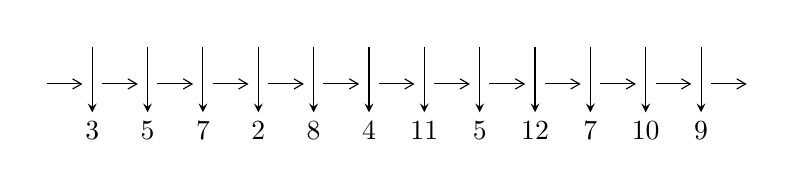
\begin{tikzpicture}[x=20pt, y=17pt]
	% nodes
	\node (C0) at (0, 0) {};
	\node (C1) at (1, 0) {};
	\node (C1U) at (1, +1) {};
	\node (C1D) at (1, -1) {3};

	\node (C2) at (2, 0) {};
	\node (C2U) at (2, +1) {};
	\node (C2D) at (2, -1) {5};

	\node (C3) at (3, 0) {};
	\node (C3U) at (3, +1) {};
	\node (C3D) at (3, -1) {7};

	\node (C4) at (4, 0) {};
	\node (C4U) at (4, +1) {};
	\node (C4D) at (4, -1) {2};

	\node (C5) at (5, 0) {};
	\node (C5U) at (5, +1) {};
	\node (C5D) at (5, -1) {8};

	\node (C6) at (6, 0) {};
	\node (C6U) at (6, +1) {};
	\node (C6D) at (6, -1) {4};

	\node (C7) at (7, 0) {};
	\node (C7U) at (7, +1) {};
	\node (C7D) at (7, -1) {11};

	\node (C8) at (8, 0) {};
	\node (C8U) at (8, +1) {};
	\node (C8D) at (8, -1) {5};

	\node (C9) at (9, 0) {};
	\node (C9U) at (9, +1) {};
	\node (C9D) at (9, -1) {12};

	\node (C10) at (10, 0) {};
	\node (C10U) at (10, +1) {};
	\node (C10D) at (10, -1) {7};

	\node (C11) at (11, 0) {};
	\node (C11U) at (11, +1) {};
	\node (C11D) at (11, -1) {10};

	\node (C12) at (12, 0) {};
	\node (C12U) at (12, +1) {};
	\node (C12D) at (12, -1) {9};
	\node (C13) at (13, 0) {};

	% arrows
	\draw[->,>={angle 60}]
	(C0) edge (C1) (C1) edge (C2) (C2) edge (C3) (C3) edge (C4) (C4) edge (C5) (C5) edge (C6) (C6) edge (C7) (C7) edge (C8) (C8) edge (C9) (C9) edge (C10) (C10) edge (C11) (C11) edge (C12) (C12) edge (C13) ;	\draw[->,>=stealth]
	(C1U) edge (C1D) (C2U) edge (C2D) (C3U) edge (C3D) (C4U) edge (C4D) (C5U) edge (C5D) (C6U) edge (C6D) (C7U) edge (C7D) (C8U) edge (C8D) (C9U) edge (C9D) (C10U) edge (C10D) (C11U) edge (C11D) (C12U) edge (C12D) ;
	\end{tikzpicture} \\
\hhline{~~} \\& 
\textbf{Solving Sequence} \\ \cline{2-2} 
 &
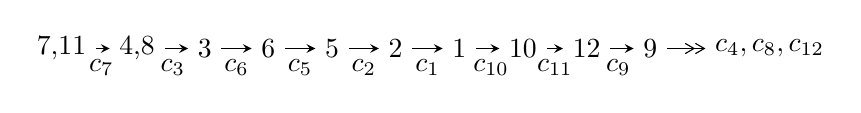
\begin{tikzpicture}[x=23pt, y=7pt]
	% node
	\node (A0) at (-1/8, 0) {7,11};
	\node (A1) at (17/16, 0) {4,8};
	\node (A2) at (17/8, 0) {3};
	\node (A3) at (25/8, 0) {6};
	\node (A4) at (33/8, 0) {5};
	\node (A5) at (41/8, 0) {2};
	\node (A6) at (49/8, 0) {1};
	\node (A7) at (57/8, 0) {10};
	\node (A8) at (65/8, 0) {12};
	\node (A9) at (73/8, 0) {9};
	\node (C1) at (1/2, -1) {$c_{7}$};
	\node (C2) at (13/8, -1) {$c_{3}$};
	\node (C3) at (21/8, -1) {$c_{6}$};
	\node (C4) at (29/8, -1) {$c_{5}$};
	\node (C5) at (37/8, -1) {$c_{2}$};
	\node (C6) at (45/8, -1) {$c_{1}$};
	\node (C7) at (53/8, -1) {$c_{10}$};
	\node (C8) at (61/8, -1) {$c_{11}$};
	\node (C9) at (69/8, -1) {$c_{9}$};
	\node (A10) at (11, 0) {$c_{4},c_{8},c_{12}$};

	% edge
	\draw[->,>=stealth]	
	(A0) edge (A1) (A1) edge (A2) (A2) edge (A3) (A3) edge (A4) (A4) edge (A5) (A5) edge (A6) (A6) edge (A7) (A7) edge (A8) (A8) edge (A9) ;
	\draw[->>,>={angle 60}]	
	(A9) edge (A10);
\end{tikzpicture} \\ 

\end{tabular} \\

\footnotetext{
The image of knot diagram is generated by the software ``\textbf{Draw programme}" developed by Andrew Bartholomew(\url{http://www.layer8.co.uk/maths/draw/index.htm\#Running-draw}), where we modified some parts for our purpose(\url{https://github.com/CATsTAILs/LinksPainter}).
}\phantom \\ \newline 
\centering \textbf{Ideals for irreducible components\footnotemark of $X_{\text{par}}$} 
 
\begin{align*}
I^u_{1}&=\langle 
-4915 u^{16}+20254 u^{15}+\cdots+7156 b+9167,\;-123805 u^{16}+530300 u^{15}+\cdots+7156 a+154261,\\
\phantom{I^u_{1}}&\phantom{= \langle  }u^{17}-5 u^{16}+\cdots-9 u+1\rangle \\
I^u_{2}&=\langle 
u^2+b,\;a+u+2,\;u^3+u^2-1\rangle \\
I^u_{3}&=\langle 
b,\;3 u^4- u^3- u^2+a+3 u+4,\;u^5- u^4+u^2+u-1\rangle \\
I^u_{4}&=\langle 
-3 u^2 a-2 a u-4 u^2+5 b- a- u+2,\;a^2+2 u^2+a+2 u,\;u^3+u^2-1\rangle \\
\\
\end{align*}
\raggedright * 4 irreducible components of $\dim_{\mathbb{C}}=0$, with total 31 representations.\\
\footnotetext{All coefficients of polynomials are rational numbers. But the coefficients are sometimes approximated in decimal forms when there is not enough margin.}
\newpage
\renewcommand{\arraystretch}{1}
\centering \section*{I. $I^u_{1}= \langle -4915 u^{16}+20254 u^{15}+\cdots+7156 b+9167,\;-1.24\times10^{5} u^{16}+5.30\times10^{5} u^{15}+\cdots+7156 a+1.54\times10^{5},\;u^{17}-5 u^{16}+\cdots-9 u+1 \rangle$}
\flushleft \textbf{(i) Arc colorings}\\
\begin{tabular}{m{7pt} m{180pt} m{7pt} m{180pt} }
\flushright $a_{7}=$&$\begin{pmatrix}1\\0\end{pmatrix}$ \\
\flushright $a_{11}=$&$\begin{pmatrix}0\\u\end{pmatrix}$ \\
\flushright $a_{4}=$&$\begin{pmatrix}17.3009 u^{16}-74.1056 u^{15}+\cdots+179.512 u-21.5569\\0.686836 u^{16}-2.83035 u^{15}+\cdots+5.34754 u-1.28102\end{pmatrix}$ \\
\flushright $a_{8}=$&$\begin{pmatrix}1\\u^2\end{pmatrix}$ \\
\flushright $a_{3}=$&$\begin{pmatrix}17.9877 u^{16}-76.9360 u^{15}+\cdots+184.860 u-22.8379\\0.686836 u^{16}-2.83035 u^{15}+\cdots+5.34754 u-1.28102\end{pmatrix}$ \\
\flushright $a_{6}=$&$\begin{pmatrix}-4.26593 u^{16}+18.3215 u^{15}+\cdots-48.9090 u+8.75545\\-0.297652 u^{16}+1.56051 u^{15}+\cdots-5.66867 u+0.378144\end{pmatrix}$ \\
\flushright $a_{5}=$&$\begin{pmatrix}-2.46297 u^{16}+10.6539 u^{15}+\cdots-31.7707 u+6.12549\\0.563164 u^{16}-2.41965 u^{15}+\cdots+4.65246 u-0.968977\end{pmatrix}$ \\
\flushright $a_{2}=$&$\begin{pmatrix}18.8118 u^{16}-80.6283 u^{15}+\cdots+197.318 u-25.5869\\0.563164 u^{16}-2.41965 u^{15}+\cdots+4.65246 u-0.968977\end{pmatrix}$ \\
\flushright $a_{1}=$&$\begin{pmatrix}u^7+2 u^3\\u^7- u^5+2 u^3- u\end{pmatrix}$ \\
\flushright $a_{10}=$&$\begin{pmatrix}u\\u\end{pmatrix}$ \\
\flushright $a_{12}=$&$\begin{pmatrix}- u^3\\- u^3+u\end{pmatrix}$ \\
\flushright $a_{9}=$&$\begin{pmatrix}u^5+u\\u^5- u^3+u\end{pmatrix}$\\&\end{tabular}
\flushleft \textbf{(ii) Obstruction class $= -1$}\\~\\
\flushleft \textbf{(iii) Cusp Shapes $= -\frac{440209}{1789} u^{16}+\frac{7557829}{7156} u^{15}+\cdots-\frac{18828293}{7156} u+\frac{602132}{1789}$}\\~\\
\newpage\renewcommand{\arraystretch}{1}
\flushleft \textbf{(iv) u-Polynomials at the component}\newline \\
\begin{tabular}{m{50pt}|m{274pt}}
Crossings & \hspace{64pt}u-Polynomials at each crossing \\
\hline $$\begin{aligned}c_{1}\end{aligned}$$&$\begin{aligned}
&u^{17}+25 u^{16}+\cdots+349 u+1
\end{aligned}$\\
\hline $$\begin{aligned}c_{2},c_{4}\end{aligned}$$&$\begin{aligned}
&u^{17}-9 u^{16}+\cdots-23 u-1
\end{aligned}$\\
\hline $$\begin{aligned}c_{3},c_{6}\end{aligned}$$&$\begin{aligned}
&u^{17}-4 u^{16}+\cdots-808 u^2+32
\end{aligned}$\\
\hline $$\begin{aligned}c_{5},c_{8}\end{aligned}$$&$\begin{aligned}
&u^{17}-9 u^{16}+\cdots+1536 u+512
\end{aligned}$\\
\hline $$\begin{aligned}c_{7},c_{10}\end{aligned}$$&$\begin{aligned}
&u^{17}+5 u^{16}+\cdots-9 u-1
\end{aligned}$\\
\hline $$\begin{aligned}c_{9},c_{11},c_{12}\end{aligned}$$&$\begin{aligned}
&u^{17}+9 u^{16}+\cdots+19 u+1
\end{aligned}$\\
\hline
\end{tabular}\\~\\
\newpage\renewcommand{\arraystretch}{1}
\flushleft \textbf{(v) Riley Polynomials at the component}\newline \\
\begin{tabular}{m{50pt}|m{274pt}}
Crossings & \hspace{64pt}Riley Polynomials at each crossing \\
\hline $$\begin{aligned}c_{1}\end{aligned}$$&$\begin{aligned}
&y^{17}-57 y^{16}+\cdots+110253 y-1
\end{aligned}$\\
\hline $$\begin{aligned}c_{2},c_{4}\end{aligned}$$&$\begin{aligned}
&y^{17}-25 y^{16}+\cdots+349 y-1
\end{aligned}$\\
\hline $$\begin{aligned}c_{3},c_{6}\end{aligned}$$&$\begin{aligned}
&y^{17}-48 y^{16}+\cdots+51712 y-1024
\end{aligned}$\\
\hline $$\begin{aligned}c_{5},c_{8}\end{aligned}$$&$\begin{aligned}
&y^{17}-49 y^{16}+\cdots+4063232 y-262144
\end{aligned}$\\
\hline $$\begin{aligned}c_{7},c_{10}\end{aligned}$$&$\begin{aligned}
&y^{17}-9 y^{16}+\cdots+19 y-1
\end{aligned}$\\
\hline $$\begin{aligned}c_{9},c_{11},c_{12}\end{aligned}$$&$\begin{aligned}
&y^{17}+3 y^{16}+\cdots-149 y-1
\end{aligned}$\\
\hline
\end{tabular}\\~\\
\newpage\flushleft \textbf{(vi) Complex Volumes and Cusp Shapes}
$$\begin{array}{c|c|c}  
\text{Solutions to }I^u_{1}& \I (\text{vol} + \sqrt{-1}CS) & \text{Cusp shape}\\
 \hline 
\begin{aligned}
u &= -0.838900 + 0.274006 I \\
a &= -0.541331 + 1.242290 I \\
b &= \phantom{-}0.022802 + 1.171600 I\end{aligned}
 & \phantom{-}1.70067 + 3.40197 I & -9.83492 - 9.12548 I \\ \hline\begin{aligned}
u &= -0.838900 - 0.274006 I \\
a &= -0.541331 - 1.242290 I \\
b &= \phantom{-}0.022802 - 1.171600 I\end{aligned}
 & \phantom{-}1.70067 - 3.40197 I & -9.83492 + 9.12548 I \\ \hline\begin{aligned}
u &= -0.888050 + 0.699587 I \\
a &= \phantom{-}0.963662 + 0.607402 I \\
b &= \phantom{-}0.599165 + 0.085043 I\end{aligned}
 & \phantom{-}2.22871 + 2.69541 I & -2.36795 - 0.48316 I \\ \hline\begin{aligned}
u &= -0.888050 - 0.699587 I \\
a &= \phantom{-}0.963662 - 0.607402 I \\
b &= \phantom{-}0.599165 - 0.085043 I\end{aligned}
 & \phantom{-}2.22871 - 2.69541 I & -2.36795 + 0.48316 I \\ \hline\begin{aligned}
u &= \phantom{-}0.702958\phantom{ +0.000000I} \\
a &= \phantom{-}8.08327\phantom{ +0.000000I} \\
b &= \phantom{-}0.212168\phantom{ +0.000000I}\end{aligned}
 & -2.60036\phantom{ +0.000000I} & -117.690\phantom{ +0.000000I} \\ \hline\begin{aligned}
u &= \phantom{-}0.638788 + 1.195210 I \\
a &= -0.615352 + 0.257656 I \\
b &= \phantom{-}2.18853 - 1.40547 I\end{aligned}
 & -10.83360 + 4.83632 I & -9.98493 - 0.99160 I \\ \hline\begin{aligned}
u &= \phantom{-}0.638788 - 1.195210 I \\
a &= -0.615352 - 0.257656 I \\
b &= \phantom{-}2.18853 + 1.40547 I\end{aligned}
 & -10.83360 - 4.83632 I & -9.98493 + 0.99160 I \\ \hline\begin{aligned}
u &= \phantom{-}0.932524 + 0.992733 I \\
a &= \phantom{-}0.024900 + 0.723358 I \\
b &= -1.316500 - 0.396988 I\end{aligned}
 & \phantom{-}8.46454 - 3.58781 I & -11.43442 + 3.20089 I \\ \hline\begin{aligned}
u &= \phantom{-}0.932524 - 0.992733 I \\
a &= \phantom{-}0.024900 - 0.723358 I \\
b &= -1.316500 + 0.396988 I\end{aligned}
 & \phantom{-}8.46454 + 3.58781 I & -11.43442 - 3.20089 I \\ \hline\begin{aligned}
u &= \phantom{-}0.596043\phantom{ +0.000000I} \\
a &= \phantom{-}0.723994\phantom{ +0.000000I} \\
b &= -0.233910\phantom{ +0.000000I}\end{aligned}
 & -0.842519\phantom{ +0.000000I} & -11.7040\phantom{ +0.000000I}\\
 \hline 
 \end{array}$$\newpage$$\begin{array}{c|c|c}  
\text{Solutions to }I^u_{1}& \I (\text{vol} + \sqrt{-1}CS) & \text{Cusp shape}\\
 \hline 
\begin{aligned}
u &= \phantom{-}1.18905 + 0.84637 I \\
a &= \phantom{-}1.44006 - 1.34507 I \\
b &= \phantom{-}1.69244 + 1.67258 I\end{aligned}
 & -12.6169 - 12.0697 I & -10.79554 + 4.97668 I \\ \hline\begin{aligned}
u &= \phantom{-}1.18905 - 0.84637 I \\
a &= \phantom{-}1.44006 + 1.34507 I \\
b &= \phantom{-}1.69244 - 1.67258 I\end{aligned}
 & -12.6169 + 12.0697 I & -10.79554 - 4.97668 I \\ \hline\begin{aligned}
u &= \phantom{-}1.45050 + 0.33561 I \\
a &= -1.67908 + 1.23512 I \\
b &= -2.95952 + 0.58336 I\end{aligned}
 & -4.97113 - 2.77667 I & -12.19520 + 1.72835 I \\ \hline\begin{aligned}
u &= \phantom{-}1.45050 - 0.33561 I \\
a &= -1.67908 - 1.23512 I \\
b &= -2.95952 - 0.58336 I\end{aligned}
 & -4.97113 + 2.77667 I & -12.19520 - 1.72835 I \\ \hline\begin{aligned}
u &= \phantom{-}0.248594 + 0.150644 I \\
a &= \phantom{-}1.39946 - 0.69681 I \\
b &= -0.634067 + 0.017100 I\end{aligned}
 & -0.943827 + 0.013133 I & -9.47910 + 0.58994 I \\ \hline\begin{aligned}
u &= \phantom{-}0.248594 - 0.150644 I \\
a &= \phantom{-}1.39946 + 0.69681 I \\
b &= -0.634067 - 0.017100 I\end{aligned}
 & -0.943827 - 0.013133 I & -9.47910 - 0.58994 I \\ \hline\begin{aligned}
u &= -1.76401\phantom{ +0.000000I} \\
a &= \phantom{-}2.20808\phantom{ +0.000000I} \\
b &= \phantom{-}4.83602\phantom{ +0.000000I}\end{aligned}
 & \phantom{-}19.2915\phantom{ +0.000000I} & -12.4240\phantom{ +0.000000I}\\
 \hline 
 \end{array}$$\newpage\newpage\renewcommand{\arraystretch}{1}
\centering \section*{II. $I^u_{2}= \langle u^2+b,\;a+u+2,\;u^3+u^2-1 \rangle$}
\flushleft \textbf{(i) Arc colorings}\\
\begin{tabular}{m{7pt} m{180pt} m{7pt} m{180pt} }
\flushright $a_{7}=$&$\begin{pmatrix}1\\0\end{pmatrix}$ \\
\flushright $a_{11}=$&$\begin{pmatrix}0\\u\end{pmatrix}$ \\
\flushright $a_{4}=$&$\begin{pmatrix}- u-2\\- u^2\end{pmatrix}$ \\
\flushright $a_{8}=$&$\begin{pmatrix}1\\u^2\end{pmatrix}$ \\
\flushright $a_{3}=$&$\begin{pmatrix}- u^2- u-2\\- u^2\end{pmatrix}$ \\
\flushright $a_{6}=$&$\begin{pmatrix}- u^2\\- u^2- u+1\end{pmatrix}$ \\
\flushright $a_{5}=$&$\begin{pmatrix}- u^2\\- u^2- u+1\end{pmatrix}$ \\
\flushright $a_{2}=$&$\begin{pmatrix}-2 u^2- u-1\\- u^2- u+1\end{pmatrix}$ \\
\flushright $a_{1}=$&$\begin{pmatrix}-1\\0\end{pmatrix}$ \\
\flushright $a_{10}=$&$\begin{pmatrix}u\\u\end{pmatrix}$ \\
\flushright $a_{12}=$&$\begin{pmatrix}u^2-1\\u^2+u-1\end{pmatrix}$ \\
\flushright $a_{9}=$&$\begin{pmatrix}1\\u^2\end{pmatrix}$\\&\end{tabular}
\flushleft \textbf{(ii) Obstruction class $= 1$}\\~\\
\flushleft \textbf{(iii) Cusp Shapes $= 2 u^2-5 u-14$}\\~\\
\newpage\renewcommand{\arraystretch}{1}
\flushleft \textbf{(iv) u-Polynomials at the component}\newline \\
\begin{tabular}{m{50pt}|m{274pt}}
Crossings & \hspace{64pt}u-Polynomials at each crossing \\
\hline $$\begin{aligned}c_{1},c_{3},c_{9}\end{aligned}$$&$\begin{aligned}
&u^3- u^2+2 u-1
\end{aligned}$\\
\hline $$\begin{aligned}c_{2},c_{7}\end{aligned}$$&$\begin{aligned}
&u^3+u^2-1
\end{aligned}$\\
\hline $$\begin{aligned}c_{4},c_{10}\end{aligned}$$&$\begin{aligned}
&u^3- u^2+1
\end{aligned}$\\
\hline $$\begin{aligned}c_{5},c_{8}\end{aligned}$$&$\begin{aligned}
&u^3
\end{aligned}$\\
\hline $$\begin{aligned}c_{6},c_{11},c_{12}\end{aligned}$$&$\begin{aligned}
&u^3+u^2+2 u+1
\end{aligned}$\\
\hline
\end{tabular}\\~\\
\newpage\renewcommand{\arraystretch}{1}
\flushleft \textbf{(v) Riley Polynomials at the component}\newline \\
\begin{tabular}{m{50pt}|m{274pt}}
Crossings & \hspace{64pt}Riley Polynomials at each crossing \\
\hline $$\begin{aligned}c_{1},c_{3},c_{6}\\c_{9},c_{11},c_{12}\end{aligned}$$&$\begin{aligned}
&y^3+3 y^2+2 y-1
\end{aligned}$\\
\hline $$\begin{aligned}c_{2},c_{4},c_{7}\\c_{10}\end{aligned}$$&$\begin{aligned}
&y^3- y^2+2 y-1
\end{aligned}$\\
\hline $$\begin{aligned}c_{5},c_{8}\end{aligned}$$&$\begin{aligned}
&y^3
\end{aligned}$\\
\hline
\end{tabular}\\~\\
\newpage\flushleft \textbf{(vi) Complex Volumes and Cusp Shapes}
$$\begin{array}{c|c|c}  
\text{Solutions to }I^u_{2}& \I (\text{vol} + \sqrt{-1}CS) & \text{Cusp shape}\\
 \hline 
\begin{aligned}
u &= -0.877439 + 0.744862 I \\
a &= -1.122560 - 0.744862 I \\
b &= -0.215080 + 1.307140 I\end{aligned}
 & \phantom{-}6.04826 + 5.65624 I & -9.18265 - 6.33859 I \\ \hline\begin{aligned}
u &= -0.877439 - 0.744862 I \\
a &= -1.122560 + 0.744862 I \\
b &= -0.215080 - 1.307140 I\end{aligned}
 & \phantom{-}6.04826 - 5.65624 I & -9.18265 + 6.33859 I \\ \hline\begin{aligned}
u &= \phantom{-}0.754878\phantom{ +0.000000I} \\
a &= -2.75488\phantom{ +0.000000I} \\
b &= -0.569840\phantom{ +0.000000I}\end{aligned}
 & -2.22691\phantom{ +0.000000I} & -16.6350\phantom{ +0.000000I}\\
 \hline 
 \end{array}$$\newpage\newpage\renewcommand{\arraystretch}{1}
\centering \section*{III. $I^u_{3}= \langle b,\;3 u^4- u^3- u^2+a+3 u+4,\;u^5- u^4+u^2+u-1 \rangle$}
\flushleft \textbf{(i) Arc colorings}\\
\begin{tabular}{m{7pt} m{180pt} m{7pt} m{180pt} }
\flushright $a_{7}=$&$\begin{pmatrix}1\\0\end{pmatrix}$ \\
\flushright $a_{11}=$&$\begin{pmatrix}0\\u\end{pmatrix}$ \\
\flushright $a_{4}=$&$\begin{pmatrix}-3 u^4+u^3+u^2-3 u-4\\0\end{pmatrix}$ \\
\flushright $a_{8}=$&$\begin{pmatrix}1\\u^2\end{pmatrix}$ \\
\flushright $a_{3}=$&$\begin{pmatrix}-3 u^4+u^3+u^2-3 u-4\\0\end{pmatrix}$ \\
\flushright $a_{6}=$&$\begin{pmatrix}1\\0\end{pmatrix}$ \\
\flushright $a_{5}=$&$\begin{pmatrix}- u^2+1\\- u^4\end{pmatrix}$ \\
\flushright $a_{2}=$&$\begin{pmatrix}-3 u^4+u^3+2 u^2-3 u-5\\u^4\end{pmatrix}$ \\
\flushright $a_{1}=$&$\begin{pmatrix}u^2-1\\u^4\end{pmatrix}$ \\
\flushright $a_{10}=$&$\begin{pmatrix}u\\u\end{pmatrix}$ \\
\flushright $a_{12}=$&$\begin{pmatrix}- u^3\\- u^3+u\end{pmatrix}$ \\
\flushright $a_{9}=$&$\begin{pmatrix}u^4- u^2+1\\u^4- u^3- u^2+1\end{pmatrix}$\\&\end{tabular}
\flushleft \textbf{(ii) Obstruction class $= 1$}\\~\\
\flushleft \textbf{(iii) Cusp Shapes $= 10 u^4-7 u^3+u^2+10 u+7$}\\~\\
\newpage\renewcommand{\arraystretch}{1}
\flushleft \textbf{(iv) u-Polynomials at the component}\newline \\
\begin{tabular}{m{50pt}|m{274pt}}
Crossings & \hspace{64pt}u-Polynomials at each crossing \\
\hline $$\begin{aligned}c_{1},c_{2}\end{aligned}$$&$\begin{aligned}
&(u-1)^5
\end{aligned}$\\
\hline $$\begin{aligned}c_{3},c_{6}\end{aligned}$$&$\begin{aligned}
&u^5
\end{aligned}$\\
\hline $$\begin{aligned}c_{4}\end{aligned}$$&$\begin{aligned}
&(u+1)^5
\end{aligned}$\\
\hline $$\begin{aligned}c_{5},c_{9}\end{aligned}$$&$\begin{aligned}
&u^5- u^4+4 u^3-3 u^2+3 u-1
\end{aligned}$\\
\hline $$\begin{aligned}c_{7}\end{aligned}$$&$\begin{aligned}
&u^5- u^4+u^2+u-1
\end{aligned}$\\
\hline $$\begin{aligned}c_{8},c_{11},c_{12}\end{aligned}$$&$\begin{aligned}
&u^5+u^4+4 u^3+3 u^2+3 u+1
\end{aligned}$\\
\hline $$\begin{aligned}c_{10}\end{aligned}$$&$\begin{aligned}
&u^5+u^4- u^2+u+1
\end{aligned}$\\
\hline
\end{tabular}\\~\\
\newpage\renewcommand{\arraystretch}{1}
\flushleft \textbf{(v) Riley Polynomials at the component}\newline \\
\begin{tabular}{m{50pt}|m{274pt}}
Crossings & \hspace{64pt}Riley Polynomials at each crossing \\
\hline $$\begin{aligned}c_{1},c_{2},c_{4}\end{aligned}$$&$\begin{aligned}
&(y-1)^5
\end{aligned}$\\
\hline $$\begin{aligned}c_{3},c_{6}\end{aligned}$$&$\begin{aligned}
&y^5
\end{aligned}$\\
\hline $$\begin{aligned}c_{5},c_{8},c_{9}\\c_{11},c_{12}\end{aligned}$$&$\begin{aligned}
&y^5+7 y^4+16 y^3+13 y^2+3 y-1
\end{aligned}$\\
\hline $$\begin{aligned}c_{7},c_{10}\end{aligned}$$&$\begin{aligned}
&y^5- y^4+4 y^3-3 y^2+3 y-1
\end{aligned}$\\
\hline
\end{tabular}\\~\\
\newpage\flushleft \textbf{(vi) Complex Volumes and Cusp Shapes}
$$\begin{array}{c|c|c}  
\text{Solutions to }I^u_{3}& \I (\text{vol} + \sqrt{-1}CS) & \text{Cusp shape}\\
 \hline 
\begin{aligned}
u &= -0.758138 + 0.584034 I \\
a &= \phantom{-}1.036940 - 0.588205 I \\
b &= \phantom{-0.000000 } 0\end{aligned}
 & \phantom{-}0.17487 + 2.21397 I & -10.02401 - 4.83884 I \\ \hline\begin{aligned}
u &= -0.758138 - 0.584034 I \\
a &= \phantom{-}1.036940 + 0.588205 I \\
b &= \phantom{-0.000000 } 0\end{aligned}
 & \phantom{-}0.17487 - 2.21397 I & -10.02401 + 4.83884 I \\ \hline\begin{aligned}
u &= \phantom{-}0.935538 + 0.903908 I \\
a &= \phantom{-}0.348360 + 0.023996 I \\
b &= \phantom{-0.000000 } 0\end{aligned}
 & \phantom{-}9.31336 - 3.33174 I & -1.83654 + 1.25445 I \\ \hline\begin{aligned}
u &= \phantom{-}0.935538 - 0.903908 I \\
a &= \phantom{-}0.348360 - 0.023996 I \\
b &= \phantom{-0.000000 } 0\end{aligned}
 & \phantom{-}9.31336 + 3.33174 I & -1.83654 - 1.25445 I \\ \hline\begin{aligned}
u &= \phantom{-}0.645200\phantom{ +0.000000I} \\
a &= -5.77061\phantom{ +0.000000I} \\
b &= \phantom{-0.000000 } 0\end{aligned}
 & -2.52712\phantom{ +0.000000I} & \phantom{-}13.7210\phantom{ +0.000000I}\\
 \hline 
 \end{array}$$\newpage\newpage\renewcommand{\arraystretch}{1}
\centering \section*{IV. $I^u_{4}= \langle -3 u^2 a-2 a u-4 u^2+5 b- a- u+2,\;a^2+2 u^2+a+2 u,\;u^3+u^2-1 \rangle$}
\flushleft \textbf{(i) Arc colorings}\\
\begin{tabular}{m{7pt} m{180pt} m{7pt} m{180pt} }
\flushright $a_{7}=$&$\begin{pmatrix}1\\0\end{pmatrix}$ \\
\flushright $a_{11}=$&$\begin{pmatrix}0\\u\end{pmatrix}$ \\
\flushright $a_{4}=$&$\begin{pmatrix}a\\\frac{3}{5} u^2 a+\frac{4}{5} u^2+\cdots+\frac{1}{5} a-\frac{2}{5}\end{pmatrix}$ \\
\flushright $a_{8}=$&$\begin{pmatrix}1\\u^2\end{pmatrix}$ \\
\flushright $a_{3}=$&$\begin{pmatrix}\frac{3}{5} u^2 a+\frac{4}{5} u^2+\cdots+\frac{6}{5} a-\frac{2}{5}\\\frac{3}{5} u^2 a+\frac{4}{5} u^2+\cdots+\frac{1}{5} a-\frac{2}{5}\end{pmatrix}$ \\
\flushright $a_{6}=$&$\begin{pmatrix}-\frac{1}{5} u^2 a+\frac{2}{5} u^2+\cdots+\frac{3}{5} a+\frac{9}{5}\\\frac{1}{5} u^2 a+\frac{3}{5} u^2+\cdots+\frac{2}{5} a+\frac{6}{5}\end{pmatrix}$ \\
\flushright $a_{5}=$&$\begin{pmatrix}-\frac{1}{5} u^2 a+\frac{2}{5} u^2+\cdots+\frac{3}{5} a+\frac{9}{5}\\\frac{1}{5} u^2 a+\frac{3}{5} u^2+\cdots+\frac{2}{5} a+\frac{6}{5}\end{pmatrix}$ \\
\flushright $a_{2}=$&$\begin{pmatrix}u^2+a+2 u+1\\\frac{1}{5} u^2 a+\frac{3}{5} u^2+\cdots+\frac{2}{5} a+\frac{6}{5}\end{pmatrix}$ \\
\flushright $a_{1}=$&$\begin{pmatrix}-1\\0\end{pmatrix}$ \\
\flushright $a_{10}=$&$\begin{pmatrix}u\\u\end{pmatrix}$ \\
\flushright $a_{12}=$&$\begin{pmatrix}u^2-1\\u^2+u-1\end{pmatrix}$ \\
\flushright $a_{9}=$&$\begin{pmatrix}1\\u^2\end{pmatrix}$\\&\end{tabular}
\flushleft \textbf{(ii) Obstruction class $= 1$}\\~\\
\flushleft \textbf{(iii) Cusp Shapes $= -\frac{13}{5} u^2 a-\frac{17}{5} a u+\frac{26}{5} u^2+\frac{29}{5} a+\frac{24}{5} u-\frac{58}{5}$}\\~\\
\newpage\renewcommand{\arraystretch}{1}
\flushleft \textbf{(iv) u-Polynomials at the component}\newline \\
\begin{tabular}{m{50pt}|m{274pt}}
Crossings & \hspace{64pt}u-Polynomials at each crossing \\
\hline $$\begin{aligned}c_{1},c_{3},c_{9}\end{aligned}$$&$\begin{aligned}
&(u^3- u^2+2 u-1)^2
\end{aligned}$\\
\hline $$\begin{aligned}c_{2},c_{7}\end{aligned}$$&$\begin{aligned}
&(u^3+u^2-1)^2
\end{aligned}$\\
\hline $$\begin{aligned}c_{4},c_{10}\end{aligned}$$&$\begin{aligned}
&(u^3- u^2+1)^2
\end{aligned}$\\
\hline $$\begin{aligned}c_{5},c_{8}\end{aligned}$$&$\begin{aligned}
&u^6
\end{aligned}$\\
\hline $$\begin{aligned}c_{6},c_{11},c_{12}\end{aligned}$$&$\begin{aligned}
&(u^3+u^2+2 u+1)^2
\end{aligned}$\\
\hline
\end{tabular}\\~\\
\newpage\renewcommand{\arraystretch}{1}
\flushleft \textbf{(v) Riley Polynomials at the component}\newline \\
\begin{tabular}{m{50pt}|m{274pt}}
Crossings & \hspace{64pt}Riley Polynomials at each crossing \\
\hline $$\begin{aligned}c_{1},c_{3},c_{6}\\c_{9},c_{11},c_{12}\end{aligned}$$&$\begin{aligned}
&(y^3+3 y^2+2 y-1)^2
\end{aligned}$\\
\hline $$\begin{aligned}c_{2},c_{4},c_{7}\\c_{10}\end{aligned}$$&$\begin{aligned}
&(y^3- y^2+2 y-1)^2
\end{aligned}$\\
\hline $$\begin{aligned}c_{5},c_{8}\end{aligned}$$&$\begin{aligned}
&y^6
\end{aligned}$\\
\hline
\end{tabular}\\~\\
\newpage\flushleft \textbf{(vi) Complex Volumes and Cusp Shapes}
$$\begin{array}{c|c|c}  
\text{Solutions to }I^u_{4}& \I (\text{vol} + \sqrt{-1}CS) & \text{Cusp shape}\\
 \hline 
\begin{aligned}
u &= -0.877439 + 0.744862 I \\
a &= \phantom{-}0.824718 + 0.424452 I \\
b &= -0.215080 - 1.307140 I\end{aligned}
 & \phantom{-}6.04826\phantom{ +0.000000I} & -8.27833 + 0.98317 I \\ \hline\begin{aligned}
u &= -0.877439 + 0.744862 I \\
a &= -1.82472 - 0.42445 I \\
b &= -0.569840\phantom{ +0.000000I}\end{aligned}
 & \phantom{-}1.91067 + 2.82812 I & -29.3323 - 8.2928 I \\ \hline\begin{aligned}
u &= -0.877439 - 0.744862 I \\
a &= \phantom{-}0.824718 - 0.424452 I \\
b &= -0.215080 + 1.307140 I\end{aligned}
 & \phantom{-}6.04826\phantom{ +0.000000I} & -8.27833 - 0.98317 I \\ \hline\begin{aligned}
u &= -0.877439 - 0.744862 I \\
a &= -1.82472 + 0.42445 I \\
b &= -0.569840\phantom{ +0.000000I}\end{aligned}
 & \phantom{-}1.91067 - 2.82812 I & -29.3323 + 8.2928 I \\ \hline\begin{aligned}
u &= \phantom{-}0.754878\phantom{ +0.000000I} \\
a &= -0.50000 + 1.54901 I \\
b &= -0.215080 + 1.307140 I\end{aligned}
 & \phantom{-}1.91067 + 2.82812 I & -5.88933 + 2.71361 I \\ \hline\begin{aligned}
u &= \phantom{-}0.754878\phantom{ +0.000000I} \\
a &= -0.50000 - 1.54901 I \\
b &= -0.215080 - 1.307140 I\end{aligned}
 & \phantom{-}1.91067 - 2.82812 I & -5.88933 - 2.71361 I\\
 \hline 
 \end{array}$$\newpage
\newpage\renewcommand{\arraystretch}{1}
\centering \section*{ V. u-Polynomials}
\begin{tabular}{m{50pt}|m{274pt}}
Crossings & \hspace{64pt}u-Polynomials at each crossing \\
\hline $$\begin{aligned}c_{1}\end{aligned}$$&$\begin{aligned}
&((u-1)^5)(u^3- u^2+2 u-1)^3(u^{17}+25 u^{16}+\cdots+349 u+1)
\end{aligned}$\\
\hline $$\begin{aligned}c_{2}\end{aligned}$$&$\begin{aligned}
&((u-1)^5)(u^3+u^2-1)^3(u^{17}-9 u^{16}+\cdots-23 u-1)
\end{aligned}$\\
\hline $$\begin{aligned}c_{3}\end{aligned}$$&$\begin{aligned}
&u^5(u^3- u^2+2 u-1)^3(u^{17}-4 u^{16}+\cdots-808 u^{2}+32)
\end{aligned}$\\
\hline $$\begin{aligned}c_{4}\end{aligned}$$&$\begin{aligned}
&((u+1)^5)(u^3- u^2+1)^3(u^{17}-9 u^{16}+\cdots-23 u-1)
\end{aligned}$\\
\hline $$\begin{aligned}c_{5}\end{aligned}$$&$\begin{aligned}
&u^9(u^5- u^4+\cdots+3 u-1)(u^{17}-9 u^{16}+\cdots+1536 u+512)
\end{aligned}$\\
\hline $$\begin{aligned}c_{6}\end{aligned}$$&$\begin{aligned}
&u^5(u^3+u^2+2 u+1)^3(u^{17}-4 u^{16}+\cdots-808 u^{2}+32)
\end{aligned}$\\
\hline $$\begin{aligned}c_{7}\end{aligned}$$&$\begin{aligned}
&((u^3+u^2-1)^3)(u^5- u^4+u^2+u-1)(u^{17}+5 u^{16}+\cdots-9 u-1)
\end{aligned}$\\
\hline $$\begin{aligned}c_{8}\end{aligned}$$&$\begin{aligned}
&u^9(u^5+u^4+\cdots+3 u+1)(u^{17}-9 u^{16}+\cdots+1536 u+512)
\end{aligned}$\\
\hline $$\begin{aligned}c_{9}\end{aligned}$$&$\begin{aligned}
&(u^3- u^2+2 u-1)^3(u^5- u^4+4 u^3-3 u^2+3 u-1)\\
&\cdot(u^{17}+9 u^{16}+\cdots+19 u+1)
\end{aligned}$\\
\hline $$\begin{aligned}c_{10}\end{aligned}$$&$\begin{aligned}
&((u^3- u^2+1)^3)(u^5+u^4- u^2+u+1)(u^{17}+5 u^{16}+\cdots-9 u-1)
\end{aligned}$\\
\hline $$\begin{aligned}c_{11},c_{12}\end{aligned}$$&$\begin{aligned}
&(u^3+u^2+2 u+1)^3(u^5+u^4+4 u^3+3 u^2+3 u+1)\\
&\cdot(u^{17}+9 u^{16}+\cdots+19 u+1)
\end{aligned}$\\
\hline
\end{tabular}\newpage\renewcommand{\arraystretch}{1}
\centering \section*{ VI. Riley Polynomials}
\begin{tabular}{m{50pt}|m{274pt}}
Crossings & \hspace{64pt}Riley Polynomials at each crossing \\
\hline $$\begin{aligned}c_{1}\end{aligned}$$&$\begin{aligned}
&((y-1)^5)(y^3+3 y^2+2 y-1)^3(y^{17}-57 y^{16}+\cdots+110253 y-1)
\end{aligned}$\\
\hline $$\begin{aligned}c_{2},c_{4}\end{aligned}$$&$\begin{aligned}
&((y-1)^5)(y^3- y^2+2 y-1)^3(y^{17}-25 y^{16}+\cdots+349 y-1)
\end{aligned}$\\
\hline $$\begin{aligned}c_{3},c_{6}\end{aligned}$$&$\begin{aligned}
&y^5(y^3+3 y^2+2 y-1)^3(y^{17}-48 y^{16}+\cdots+51712 y-1024)
\end{aligned}$\\
\hline $$\begin{aligned}c_{5},c_{8}\end{aligned}$$&$\begin{aligned}
&y^9(y^5+7 y^4+16 y^3+13 y^2+3 y-1)\\
&\cdot(y^{17}-49 y^{16}+\cdots+4063232 y-262144)
\end{aligned}$\\
\hline $$\begin{aligned}c_{7},c_{10}\end{aligned}$$&$\begin{aligned}
&(y^3- y^2+2 y-1)^3(y^5- y^4+4 y^3-3 y^2+3 y-1)\\
&\cdot(y^{17}-9 y^{16}+\cdots+19 y-1)
\end{aligned}$\\
\hline $$\begin{aligned}c_{9},c_{11},c_{12}\end{aligned}$$&$\begin{aligned}
&(y^3+3 y^2+2 y-1)^3(y^5+7 y^4+16 y^3+13 y^2+3 y-1)\\
&\cdot(y^{17}+3 y^{16}+\cdots-149 y-1)
\end{aligned}$\\
\hline
\end{tabular}
\vskip 2pc
\end{document}